% =====================================================================
%  banner-piracy.tex -- banner específico do PousadaGuide #01 (Piracy)
%  Gerar:  make banner        (-> docs/banner-piracy.png)
% =====================================================================
\documentclass[tikz,border=0pt]{standalone}
\usepackage{fontspec}
\usepackage{xcolor}
\usepackage{graphicx}
\graphicspath{{../../assets/}{../../Piracy/assets/}}

% ---- Paleta (igual à pousadaguide.cls) ------------------------------
\definecolor{pgTeal}{HTML}{01424A}
\definecolor{pgCream}{HTML}{F3EBD5}
\definecolor{pgAbyss}{HTML}{01323A}
\definecolor{pgVoid}{HTML}{00222A}
\definecolor{pgGlow}{HTML}{5FE3C9}
\definecolor{pgKhaki}{HTML}{D6C38F}
\definecolor{pgFog}{HTML}{7FA29E}

% ---- Tipografia (IBM Plex, igual aos guias) -------------------------
\newfontfamily\pgmono{IBMPlexMono}[Extension=.otf, UprightFont=*-Regular, BoldFont=*-Bold]
\newfontfamily\pgsans{IBMPlexSans}[Extension=.otf, UprightFont=*-Regular, BoldFont=*-SemiBold]
\newfontfamily\pgdisplay{IBMPlexSansCondensed}[Extension=.otf, UprightFont=*-Bold]

\newcommand\chip[3]{% #1 fundo  #2 texto  #3 rótulo
  \node[anchor=west, fill=#1, text=#2, inner xsep=9bp, inner ysep=6bp,
        font=\pgmono\bfseries\fontsize{15}{16}\selectfont] (c) at (chipx) {#3};
  \coordinate (chipx) at ([xshift=10bp]c.east);}

\begin{document}
\begin{tikzpicture}[x=1bp, y=1bp]
  \useasboundingbox (0,0) rectangle (1280,640);
  \begin{scope}
    \clip (0,0) rectangle (1280,640);

    % fundo + grade
    \fill[pgTeal] (0,0) rectangle (1280,640);
    \fill[pgAbyss, opacity=.55] (0,0) rectangle (1280,120);
    \draw[pgCream, opacity=.05, line width=.6bp, step=24] (0,0) grid (1280,640);

    % halo atrás da mascote
    \fill[pgKhaki, opacity=.06] (1035,330) circle (255);
    \draw[pgGlow, opacity=.30, line width=1.4bp] (1035,330) circle (255);
    \draw[pgGlow, opacity=.14, line width=1bp, dash pattern=on 6bp off 6bp] (1035,330) circle (300);
    \draw[pgKhaki, opacity=.15, line width=.8bp] (1035,330) circle (350);

    % mascote pirata
    \node[anchor=south, inner sep=0] at (1035,-70)
      {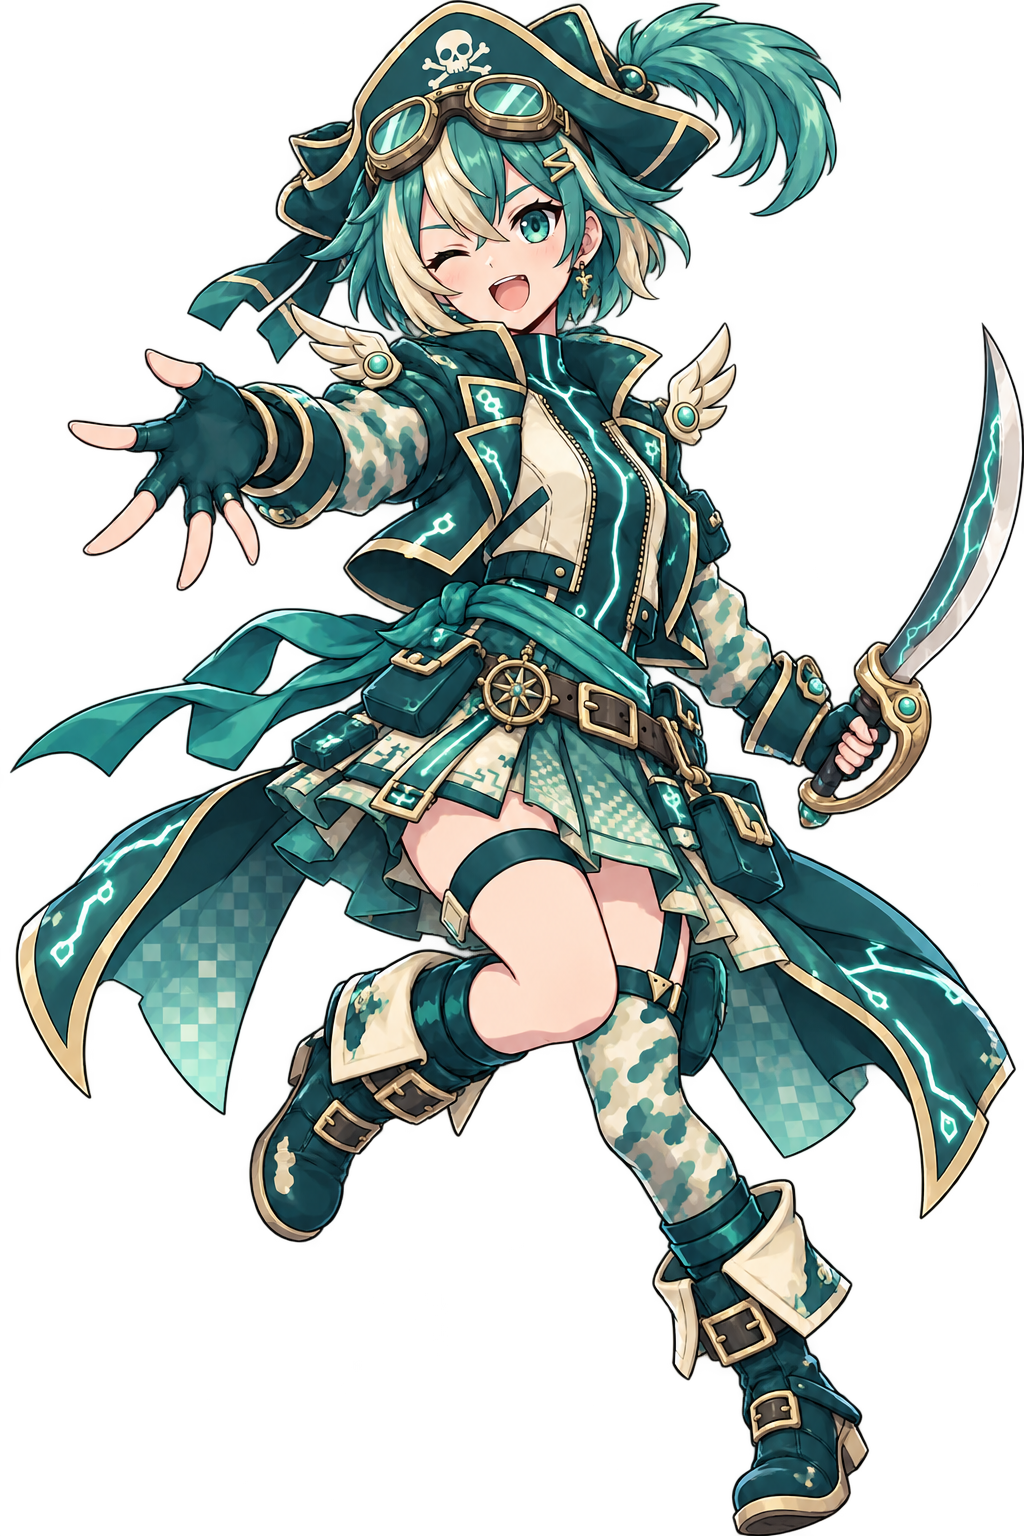
\includegraphics[height=705bp]{piracy-capa}};

    % faixa inferior
    \fill[pgGlow] (0,0) rectangle (1280,6);
  \end{scope}

  % cantos HUD
  \foreach \x/\y/\dx/\dy in {28/28/1/1, 1252/28/-1/1, 28/612/1/-1, 1252/612/-1/-1}
    \draw[pgGlow, line width=2.2bp] (\x+\dx*30,\y) -- (\x,\y) -- (\x,\y+\dy*30);

  % marca
  \node[anchor=west, inner sep=0] (logo) at (64,566)
    {
\includegraphics[height=40bp]{logo-symbol-cream}};
  \node[anchor=south west, inner sep=0, text=pgCream,
        font=\pgmono\bfseries\fontsize{17}{18}\selectfont]
    at ([xshift=16bp,yshift=1bp]logo.east) {P\,O\,U\,S\,A\,D\,A};
  \node[anchor=north west, inner sep=0, text=pgFog,
        font=\pgmono\fontsize{12}{13}\selectfont]
    at ([xshift=16bp,yshift=-3bp]logo.east) {pousadaguide // \#01};

  % rótulo + título
  \node[anchor=west, inner sep=0, text=pgGlow,
        font=\pgmono\bfseries\fontsize{20}{22}\selectfont]
    at (64,452) {>\_ pousadaguide \#01};
  \node[anchor=west, inner sep=0, text=pgCream,
        font=\pgdisplay\fontsize{98}{98}\selectfont] (t)
    at (58,370) {Piracy Guide};
  \fill[pgGlow] ([xshift=12bp,yshift=-26bp]t.east) rectangle ++(26,82);

  % subtítulo
  \node[anchor=north west, inner sep=0, text=pgCream, align=left,
        font=\pgsans\fontsize{25}{35}\selectfont]
    at (64,300) {Como navegar sem armadilhas, baixar com\\
                 segurança e dominar as \textcolor{pgGlow}{Megathreads}.};

  % chips
  \coordinate (chipx) at (64,182);
  \chip{pgKhaki}{pgVoid}{\#01 PIRACY}
  \chip{pgGlow}{pgVoid}{39 PÁG}
  \chip{pgVoid}{pgCream}{PDF}
  \chip{pgVoid}{pgCream}{MEGATHREAD}
  \chip{pgVoid}{pgCream}{OPSEC}

  % terminal
  \node[anchor=west, inner sep=0, text=pgFog,
        font=\pgmono\fontsize{15}{16}\selectfont]
    at (64,74) {\textcolor{pgGlow}{\$} make piracy \textcolor{pgGlow}{\&\&} open dist/PousadaGuide-01-Piracy.pdf};
  \node[anchor=west, inner sep=0, text=pgFog, opacity=.55,
        font=\pgmono\fontsize{10}{11}\selectfont]
    at (64,44) {00000010\quad 50 69 72 61 63 79 20 47 75 69 64 65 \quad PiracyGuide};
\end{tikzpicture}
\end{document}
